\documentclass{sig-alternate}

\usepackage[usenames,dvipsnames]{color}
\usepackage{xspace}

\usepackage{fancyvrb}
\DefineVerbatimEnvironment{code}{Verbatim}{fontsize=\small}
\DefineVerbatimEnvironment{example}{Verbatim}{fontsize=\small}

% Looks better (and more concise) than Times New Roman
\usepackage{times}
% Better spacing
\usepackage{microtype}
\usepackage[normalem]{ulem}
\usepackage{enumitem}
% Caption package both lets you set the spacing between figure and caption
% and also makes the \figref{} point to the right place.
\usepackage[font=bf,aboveskip=0pt,belowskip=-12pt]{caption}
% Get the caption package to work with ACM style
\DeclareCaptionType[placement=b,within=none]{copyrightbox}
%%%%%%%%%%%%%%%%%%%%%%%%%%%%%%%%%%%%%%%%%%%%%%%%%%%%%%%%%%%%%%%%%%%%%
\newfont{\mycrnotice}{ptmr8t at 7pt}
\newfont{\myconfname}{ptmri8t at 7pt}
\let\crnotice\mycrnotice%
\let\confname\myconfname%

\permission{Permission to make digital or hard copies of all or part of this work for personal or classroom use is granted without fee provided that copies are not made or distributed for profit or commercial advantage and that copies bear this notice and the full citation on the first page. Copyrights for components of this work owned by others than the author(s) must be honored. Abstracting with credit is permitted. To copy otherwise, or republish, to post on servers or to redistribute to lists, requires prior specific permission and/or a fee. Request permissions from Permissions@acm.org.}
\conferenceinfo{}{DMAH 2015, September 4th, Kohala Coast, USA}
\copyrightetc{}
\crdata{}

% Allow comments by name
\newcommand{\note}[2]{
    \textbf{\textcolor{#1}{#2}}
}
\newcommand{\comment}[1]{\note{red}{#1}}
\newcommand{\dave}[1]{\note{PineGreen}{Dave: #1}}
\newcommand{\magda}[1]{\note{Cyan}{Magda: #1}}
\newcommand{\tom}[1]{\note{OrangeRed}{Tom: #1}}

% To remove all notes, uncomment the next line.
%\renewcommand{\note}[2]{\unskip}

\newcommand{\ie}{{\em i.e.}\ }
\newcommand{\eg}{{\em e.g.}\ }
\newcommand{\ea}{{\em et al.}\xspace}
\newcommand{\aka}{{\em a.k.a.}\ }

\usepackage{url}
\usepackage[pdftex]{hyperref}

% Figures
\newcommand{\figureimgs}{
\begin{figure}[tbp]
  \centering
  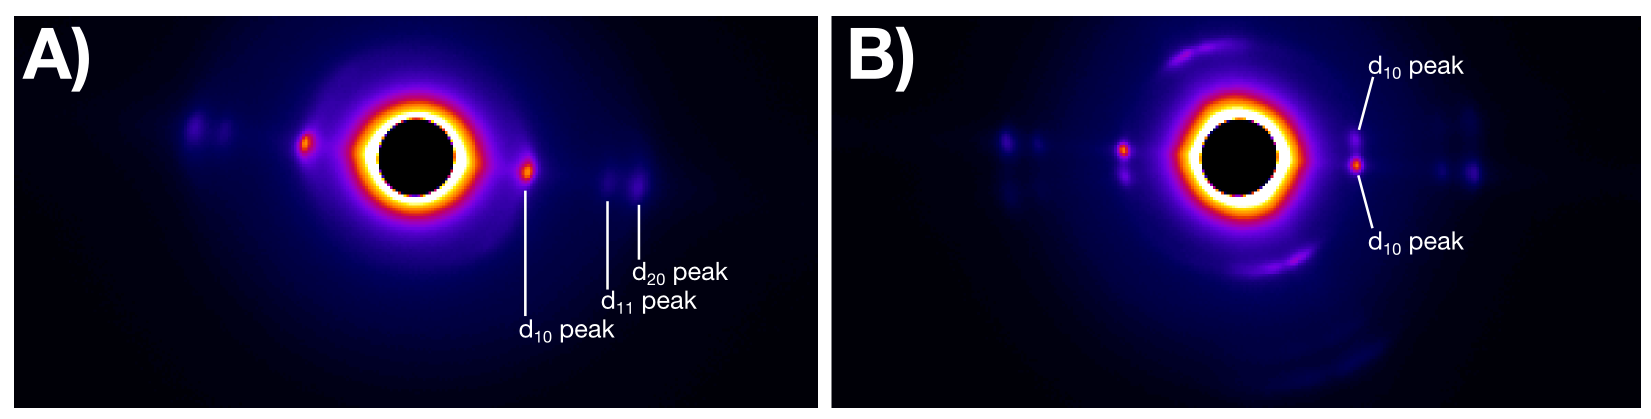
\includegraphics[width=\linewidth]{figures/x_ray_image_montage}
  \vspace{-12pt}
  \caption{\label{fig:imgs}
  	X-ray diffraction images.
    A) An X-ray diffraction image exhibits $d_{10}$, $d_{11}$, and
    $d_{20}$ peaks; the first and last are proportional to the
    distance between adjacent rows of thick filaments. B) In this
    image, two fibers at slight angles to each other have generated
    multiple $d_{10}$ peaks which must be segregated during the
    detection process.  
	}
	\vspace{-2pt}
\end{figure}
}

\newcommand{\figureworkflow}{
\begin{figure}[tbp]
  \centering
  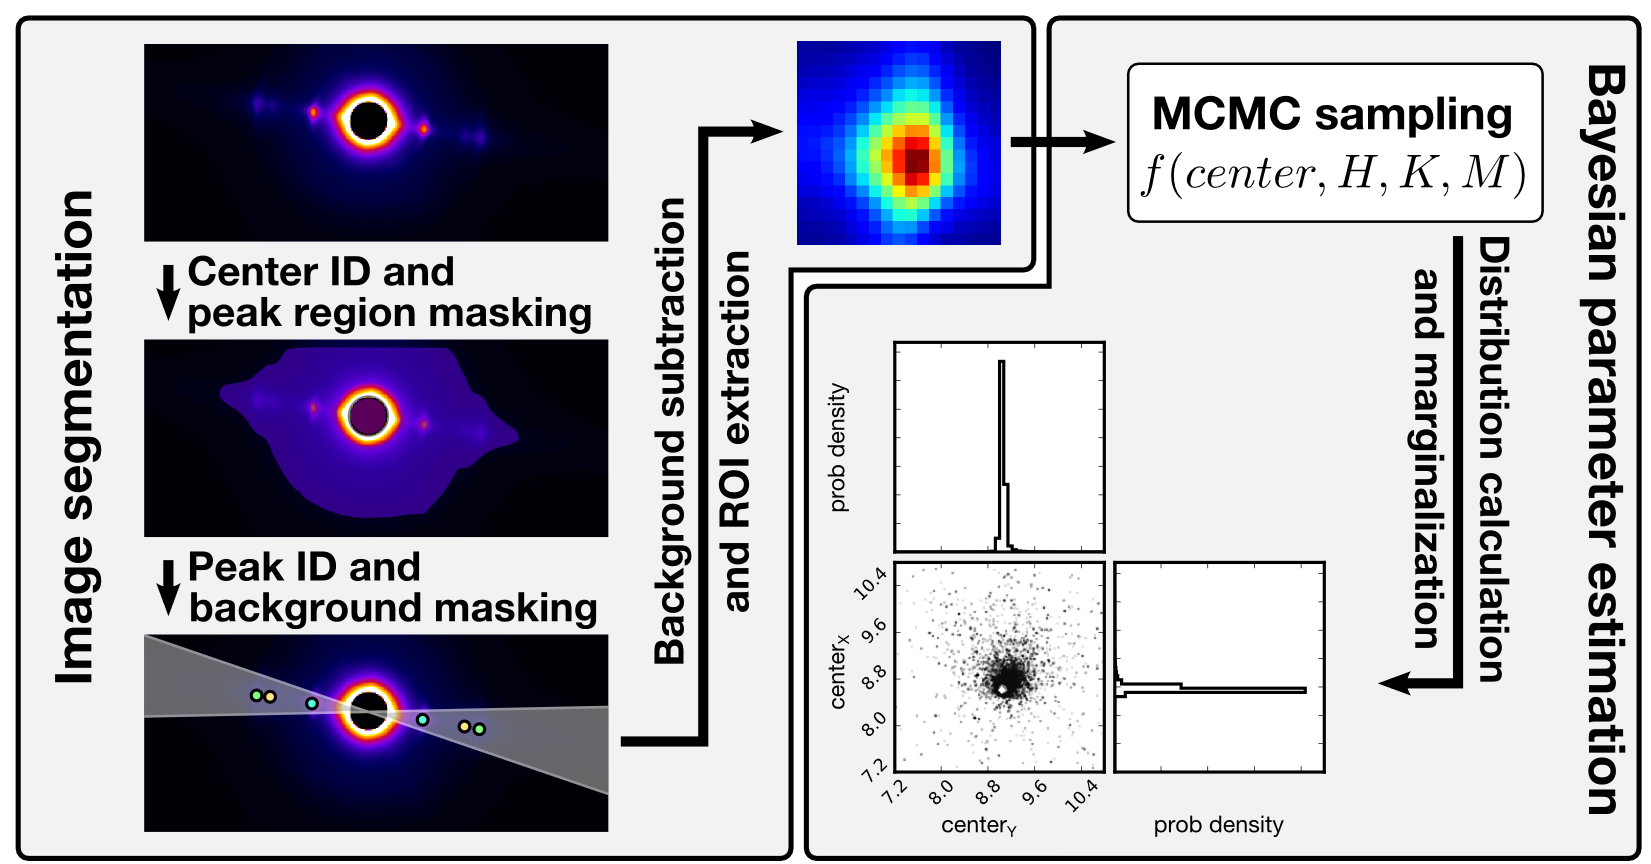
\includegraphics[width=\linewidth]{figures/img_analysis}
  \vspace{-8pt}
  \caption{\label{fig:workflow}
  	Analysis workflow.
    The blocked center region is detected and used as a landmark.  Low
    signal regions and edges are masked. The image is smoothed and
    peaks are detected, clustered, and classified. The background
    (sans that surrounding diffraction lines) is computed and
    subtracted. Regions of interest surrounding the $d_{10}$ peaks are
    extracted and the generating distributions are fit with an MCMC
    sampler. We marginalize across peak parameters other than those of
    interest.  
	}
	\vspace{-2pt}
\end{figure}
}

\begin{document}
\title{Automated Analysis of Muscle X-ray Diffraction \\ Imaging with MCMC}
\author{C.\ David Williams$^{1}$,  Magdalena Balazinska$^2$, Thomas Daniel$^1$ \\
\affaddr{$^1$Department of Biology, $^2$Department of Computer Science \& Engineering}\\
\affaddr{University of Washington} \\
}
\maketitle



% \dave{Presumably this gets filled in later?}
%    \vspace{-8pt}
%    \category{H.2.4}{Database Management}{Systems---Distributed databases, Query processing, Relational databases}
%    \vspace{-8pt}
%    \keywords{Myria; parallel data management; Cloud service; astronomy}


\sloppy

%%%%%%%%%%%
%\section{Questions addressed}
%\label{sec:addressed}


%In this work, we focus on the following questions:

%\begin{itemize}[noitemsep]
%\item Are sufficient conserved markers available in small-angle scattering diffraction images for automatic segmentation?
%\item Does MCMC distribution fitting provide reliable estimates of diffraction peak properties such as center and decay?
%\end{itemize}


%%%%%%%%%%%
\section{Motivation}
\label{sec:motivation}


The molecular regulation of force generating protein systems remains a
fundamental open problem in biology. Muscle uses a highly organized
lattice of interacting elastic and force generating molecules to
create controlled macro-scale movement \cite{Millman1998}. The advent
of advanced X-ray diffraction imaging lets us analyze protein motions
at spatial and temporal scales never previously realized, giving novel
insight into the molecular basis of motion in living systems.  

Surprisingly, we still use human experts to manually extract
structural parameters from X-ray images with NIH ImageJ. This produces
repeatable measurements but is subjective, fails to provide confidence
intervals for the measured values, and is not reproducible by naive
digitizers. Additionally hand digitization is a time-intensive
analytic technique, with a single digitizer able to process only a few
hundred images a day.  Historically this rate has been sufficient, but
new high-speed imaging systems let us investigate short-timescale
components of muscle contraction and generate data sets with many
thousands of images. The need for an automated and reproducible image
analysis tool chain is clear. 

We seek to build a service for the automated analysis of muscle
structure X-ray images. Users should specify the analysis they need
using a declarative query interface and the system should
automatically process the user's image database. In this extended
abstract, we present the first components of the processing tool chain
at the heart of this service. The toolchain first segments the
diffraction image into regions of interest using conserved features
and then samples the possible parameter values with a Markov chain
Monte Carlo approach.


%%%%%%%%%%%
\section{Prototype}
\label{sec:proto}


We initially focus on the $d_{10}$ parameter that determines the
distance which muscle's molecular motors must bridge in order to bind
and generate force \cite{Williams2013}. This distance changes during
contraction and thus regulates the force produced.

Images generated during experiments share several key features, which
serve as challenges or fiduciary marks during analysis. As seen in
Figure~\ref{fig:imgs}, the brightest part of the image background is
occluded by a circular stop. This physical block prevents damage to
the detector from the high photon flux at the center of the X-ray
beam. Surrounding the blocked region, the remainder of the image
displays an exponentially decaying background. We must locate and
model the symmetric pairs of diffraction peaks interrupting the
exponential background. Our core data analysis pipeline includes two
steps: image segmentation and image modeling with MCMC processes.

\figureimgs

\subsection{Image segmentation}

The system first identifies the dark central circular blocked region
to act as a relative landmark for subsequent operations. Consistent
with experimental design, we assume it contains the center of the
diffraction pattern. The edge of the background surrounding the block
is the brightest region, so the system first splits the image between
areas with values less than and greater than two standard deviations
above the mean. This partitioning yields a binary image where the
center blocked region is surrounded by a halo of the upper end of the
pattern background and occasional dots where diffraction peaks rise
more than two standard deviations above background. We convert this
binary image to a hierarchical contour set with OpenCV. We then take
the blocked region to be the inner-most contour and model it as the
smallest enclosing circle, shown as dark magenta in
Figure~\ref{fig:workflow}. 

With the central blocked region located, we identify local maxima in
three by three groups after Gaussian smoothing with kernel having a
three pixel standard deviation. We reject resulting maxima in regions
unlikely to provide peaks of interest before attempting to match peak
pairs. Masked rejection-regions consist of: 1) a circular zone around
the central blocked region where the blocking generates non-peak local
maxima, 2) areas below the 80th percentile where detector noise
dominates, 3) areas near the image edge where peaks are partially
cropped. The resulting unmasked area from which we keep maxima is
depicted as light purple overlay in Figure~\ref{fig:workflow}.

\figureworkflow

Next, we cluster maxima into peak pairs based on their distance and
angle from the center of the blocked region. Starting with those
maxima nearest the blocked region, a corresponding maximum is sought
an equal distance away from the blocked region and located so that the
angle formed by the two maxima and the center of the blocked region is
180$^\circ$. If no matching maximum exists within a 10\% tolerance,
the prior maximum is discarded as a spurious peak. With peak pairs now
identified (shown as color matched dots in Figure~\ref{fig:workflow}),
the diffraction center is identified by taking the mean location
between peak pairs and the background is fit and removed. 

We subtract the background by first masking arcs encompassing peak
pairs and then fitting a double exponential to a radial profile of the
remaining image. An arc swept 12$^\circ$ out on either side of each
peak pair masks the effect of the diffraction peaks on the background
(shown as a light gray arc under the peak pairs in
Figure~\ref{fig:workflow}). We calculate a radial profile of the image
around the pattern center, omitting diffraction line regions. We fit a
double exponential function of the form $background = a+ b e^{-x c} +
d e^{-x e}$ to the radial profile. From these parameters we generate
an estimated background image and subtract it from the real image,
allowing us to extract the $d{10}$ peaks as regions of interest (ROIs)
unhindered by an overlaid diffraction background.

\subsection{Image modeling with MCMC processes}

With the background subtracted and the $d_{10}$ peaks identified and
isolated from the rest of the image as ROIs, we apply Markov chain
Monte Carlo (MCMC) sampling to determine the probability distributions
from which the peak parameters could be drawn. We treat the peaks as
being drawn from an underlying Pearson VII distribution, commonly used
to fit X-ray diffraction peaks. This process allows us to generate
possible peak matches using five parameters: peak center x-location,
peak center y-location, peak height, peak spread, and peak decay rate.
We perform an initial peak fitting by residual minimization between a
generated peak and the extracted ROI. This gives a set of starting
parameters that we use, with random variation, to initialize the
positions of the MCMC agents that will explore the model space. 

Before MCMC sampling we must define our query's likelihood and prior.
We choose a flat prior as our initial information about the model is
minimal. To calculate the likelihood we represent each pixel's photon
count as a Poisson process in the form $P(d|m)=e^{-m}
\left(m^{d}/d!\right)$ where $m$ is the model value and $d$ is the
experimental data value. These functions are fed into \textit{emcee},
an efficient MCMC analysis Python library \cite{ForemanMackey2013}.
After a burn in period of 100 steps, the sampler histories are erased
and a further 1000 steps are run to generate the posterior probability
distributions of our peak parameters. 

One of MCMC modeling's convenient features is that extracting only a
subset of parameters marginalizes across those we discard. That is,
when we are interested in only the x- and y-locations of the peak
center to precisely calculate $d_{10}$ spacing (as in
Figure~\ref{fig:workflow}), we automatically integrate our uncertainty
about peak height, spread, and decay.


%%%%%%%%%%%
\section{Preliminary Evaluation}
\label{sec:eval}

We apply our workflow to a test corpus of 1,220 images generated using
X-ray diffraction during insect flight muscle research at Argonne
National Laboratory's BioCAT Beamline. Sample high-quality and
challenging images are shown in Figures~\ref{fig:imgs}A and
\ref{fig:imgs}B.  Our initial image segmentation step successfully
identifies the center blocked region of each image in greater than
99\% of images in our test corpus. The overall process allows us to
calculate peak-to-peak distances to sub-pixel accuracy with a
confidence interval of 90\%. MCMC sampling combined with image
segmentation allows us to precisely, accurately, and automatically
locate the $d_{10}$ peak centers and thus calculate the lattice
spacing measured by a diffraction image to within 0.03 nm.

Because the images in our corpus are a standard sample of those
produced by high-speed X-ray diffraction, our positive preliminary
results are a strong indication for the potential of this approach.


%%%%%%%%%%%
\section{Challenges and Next Steps}
\label{sec:challenges}

Our initial data processing pipeline produces an automated,
reproducible, objective estimate of relevant image parameters but the
following challenges remain:

\begin{itemize}[noitemsep]
\item Development of a declarative language to describe processing
    steps will speed use of this technique and ease reproducibility.
    The key question is to define the types of operations that users
    should be able to specify and how to specify them. Our goal is to
    generalize to a broad set of analysis needs for X-ray images of
    muscle structure.
\item Packaging of this tool chain into a cloud deployable
    containerized image will enable trivial scaling to work with
    larger datasets. Furthermore, the ability to access to tool chain
    directly through a web browser with automatic back-end deployment
    of the analysis pipeline will facilitate adoption. 
\item Application of these techniques to coming ultra-high
    temporal-resolution images with far lower signal:noise will strain
    autosegmentation and peak-fitting techniques. 
\end{itemize}

The increasing prevalence of advanced diffractive imaging techniques
demands data analytic methods that can handle, objectively and
reproducible, significant increases in the volume of data generated
and analyzed. This toolchain is a first step in a process that will
greatly increase the power and capabilities of a widely used approach
to understanding protein structure in living tissue. 

%%%%%%%%%%%
%\section{Acknowledgments}
%\label{sec:acknowledgments}
%
%This work was supported in part by the Army Research Office through
%ARO Grants W911NF-13-1-0435 and W911NF-14-1-0396, an award from 
%the Gordon and Betty Moore Foundation and the Alfred P Sloan 
%Foundation, the Washington Research Foundation Fund for Innovation 
%in Data-Intensive Discovery, and the UW eScience Institute.
%
%We thank Jake VanderPlas for helpful discussions of statistical
%techniques, Tom Irving for advice on X-ray imaging, and Simon Sponberg
%for the sharing of diffraction images. 


\scriptsize
\bibliography{articles,paper}
\bibliographystyle{abbrv}

\end{document}
